\chapter{The Exponential and Logarithmic Functions}

% expansion:intuition — chapter overview tying ch04 to the foundational work of ch02-ch03 and previewing what's left to make rigorous
The natural exponential function \(e^{x}\) appeared informally in Chapter 2, where we asserted its power-series form, computed its derivative \((e^{x})' = e^{x}\) by a casual term-by-term argument, and used it freely in Chapter 3 alongside its inverse \(\ln x\). This chapter goes back and grounds that informal usage rigorously: \(e^{x}\) is \emph{defined} from its power series, the convergence of that series is proved using the completeness of the real numbers, the continuity and exponent law are established as theorems, the derivative is re-derived with an explicit error bound, and \(\ln x\) is constructed as the inverse of \(e^{x}\) through a path that goes via the Mean Value Theorem. Along the way we introduce Rolle's theorem and the MVT itself --- two existence theorems that will reappear constantly in the applications chapters that follow. By the end of the chapter, every claim about \(e^{x}\) and \(\ln x\) we have used in Chapters 2 and 3 will rest on a proof.

% expansion:summary — learning outcomes distilled from the manuscript. Verb-first per CONTENT_QUICKSTART.
\paragraph{By the end of this chapter, you will be able to:}
\begin{itemize}
    \item state the power-series definition of \(e^{x}\) and bound the tail of the series to prove convergence on \(\mathbb{R}\);
    \item prove that \(e^{x}\) is continuous on \(\mathbb{R}\) and satisfies the exponent law \(e^{x} e^{y} = e^{x + y}\);
    \item re-derive \(\frac{d}{dx} e^{x} = e^{x}\) rigorously using the bound \(\bigl\lvert \frac{e^{h} - 1}{h} - 1 \bigr\rvert \leq \lvert h \rvert\) on a small interval around \(0\);
    \item state and prove Rolle's theorem and the Mean Value Theorem;
    \item use the Mean Value Theorem to establish that \(f' \geq 0\) on an interval implies \(f\) is increasing on that interval;
    \item define \(\ln x\) as the inverse of \(e^{x}\), prove its continuity, and derive \(\frac{d}{dx} \ln x = 1/x\) without circularity.
\end{itemize}

\section{Construction of the Exponential Function}\label{sec:construction-of-exp}

% expansion:intuition — section opener motivating why we go back and rebuild e^x rigorously
The natural exponential function appeared in Chapter 2 with three casual claims attached: that the series \(1 + x + x^{2}/2! + x^{3}/3! + \dots\) converges for every real \(x\), that the resulting function is continuous, and that it has the property \(e^{x} e^{y} = e^{x + y}\). All three are true but none was proved. This section starts by motivating the series definition through the algebraic build-up of \(a^{q}\) for rational \(q\), then takes the series itself as the definition of \(e^{x}\) and proves its convergence using the completeness of the real numbers. The continuity and exponent-law claims are postponed to \cref{sec:continuity-and-exponent-law}; the derivative \((e^{x})' = e^{x}\) is re-derived rigorously in \cref{sec:rigorous-derivative-of-exp}.

\subsection{From rational exponents to the series definition}

For a positive base \(a > 0\) and a positive integer \(n\), the meaning of \(a^{n}\) is obvious: it is \(a\) multiplied by itself \(n\) times. For \(n = 1/m\) with \(m\) a positive integer, \(a^{1/m}\) is defined to be the unique positive real number \(x\) with \(x^{m} = a\), the \emph{positive \(m\)-th root} of \(a\). For \(q = n/m\) a positive rational, we define
\[
a^{q} = \bigl(a^{1/m}\bigr)^{n}.
\]
The standard exponent rules \(a^{q_{1}} a^{q_{2}} = a^{q_{1} + q_{2}}\) and \(\bigl(a^{q_{1}}\bigr)^{q_{2}} = a^{q_{1} q_{2}}\) hold for all rational exponents.

The natural next question is how to define \(a^{r}\) for an \emph{irrational} \(r\). One could try to define \(a^{r}\) as a limit of \(a^{q_{n}}\) for rational sequences \(q_{n} \to r\), but this approach requires showing the limit exists and is independent of the sequence chosen. A more elegant route, and the one this chapter takes, is to define the natural exponential function \(e^{x}\) directly by a power series, then use it to define \(a^{x}\) for arbitrary positive \(a\) and arbitrary real \(x\) by \(a^{x} = e^{x \ln a}\) (the \(\ln\) construction is the subject of \cref{sec:logarithm}).

\begin{definition}\label{def:exponential-function}
For \(x \in \mathbb{R}\), the \emph{natural exponential function}\index{exponential function!definition}\index{e@$e^{x}$ (function)}\index{exponential function@$e^{x}$ (function)} is the function
\[
e^{x} = \sum_{n = 0}^{\infty} \frac{x^{n}}{n!} = 1 + x + \frac{x^{2}}{2!} + \frac{x^{3}}{3!} + \dotsb,
\]
where by convention \(0! = 1\), so the series's first term is \(1\) for every \(x\) (including \(x = 0\), where the series collapses to \(1 + 0 + 0 + \dotsb\)).

% expansion:intuition — Informally gloss
\emph{Informally, \(e^{x}\) is what you get if you take the power-series expansion the elementary calculus suggests and use it as the definition rather than as a derived consequence. This chapter will recover all the familiar properties of \(e^{x}\) from this single starting point.}
\end{definition}

% expansion:caution — the foundational shift students may miss
\begin{caution}
The series defines \(e^{x}\); it is not a property of an independently-defined \(e^{x}\) that we are merely reporting. Any property of \(e^{x}\) we want to use --- continuity, the exponent law, the derivative formula --- must be \emph{proved} from this definition, not assumed from previous experience. In particular, the informal derivation in \cref{thm:derivative-of-exp} (Chapter 2) used the series in this same role, but the convergence and continuity questions were postponed; this chapter pays them off.
\end{caution}

The first technical question is whether the series even converges. We prove convergence in two steps, first for \(x > 0\) (where the easier tail bound applies), then extending to \(x < 0\) using a slightly more refined argument that requires the absolute-convergence property in \cref{sec:continuity-and-exponent-law}.

\subsection{The completeness property}

The convergence proof for the series \(\sum x^{n}/n!\) rests on a structural property of the real numbers: every monotone bounded sequence has a limit.

\begin{theorem}[Completeness]\label{thm:completeness}\index{completeness of $\mathbb{R}$}\index{completeness}
Suppose \(\{a_{n}\}_{n = 1}^{\infty}\) is a sequence of real numbers.
\begin{enumerate}
    \item If \(a_{1} \leq a_{2} \leq \dotsb \leq a_{n} \leq \dotsb \leq M\) is non-decreasing and bounded above by some \(M \in \mathbb{R}\), then \(\lim_{n \to \infty} a_{n}\) exists.
    \item If \(a_{1} \geq a_{2} \geq \dotsb \geq a_{n} \geq \dotsb \geq L\) is non-increasing and bounded below by some \(L \in \mathbb{R}\), then \(\lim_{n \to \infty} a_{n}\) exists.
\end{enumerate}
\end{theorem}

% expansion:intuition — completeness is the analytic backbone of every existence proof in calculus; flagging this helps students see why we're invoking it
\begin{remark}
\Cref{thm:completeness} is the analytic content of what distinguishes \(\mathbb{R}\) from \(\mathbb{Q}\): the rational numbers are not complete (the sequence \(3, 3.1, 3.14, 3.141, \dots\) is non-decreasing and bounded above by \(4\) within \(\mathbb{Q}\) but has no rational limit), and many of calculus's existence theorems --- the existence of \(\lim a_{n}\), the existence of suprema and infima, the existence of solutions to \(x^{n} = a\) --- ultimately rest on this property. We will use it here to prove the series \(\sum x^{n}/n!\) converges.
\end{remark}

\subsection{Convergence of the exponential series for \texorpdfstring{$x > 0$}{x > 0}}

The strategy is to bound the tail of the series geometrically, so the partial sums form a non-decreasing bounded sequence and \cref{thm:completeness} delivers the limit.

% expansion:strategy — the tail-bound argument is reused several times in §4.1 and §4.2; naming it once makes the later occurrences immediate
\begin{strategy}[Bounding a series by a geometric tail]
To show that a series of positive terms \(\sum a_{n}\) converges, find an index \(n_{0}\) past which the ratio \(a_{n + 1}/a_{n}\) is at most some constant \(r < 1\). Then for \(n > n_{0}\), \(a_{n} \leq a_{n_{0}} \cdot r^{n - n_{0}}\), and the tail \(\sum_{n > n_{0}} a_{n}\) is bounded by the geometric tail \(a_{n_{0}} \cdot \sum_{k \geq 1} r^{k} = a_{n_{0}} \cdot r/(1 - r) < \infty\). The partial sums of the original series are therefore bounded; if they are also non-decreasing (which holds for series of positive terms), \cref{thm:completeness} gives the limit.
\end{strategy}

\begin{theorem}\label{thm:exp-series-converges-positive}
For every \(x > 0\), the series \(\sum_{n = 0}^{\infty} x^{n}/n!\) converges to a finite real number.
\end{theorem}

\begin{proof}
Fix \(x > 0\), and choose any positive integer \(n_{0}\) with \(n_{0} > 2x\). The ratio of successive terms is
\[
\frac{x^{n + 1}/(n + 1)!}{x^{n}/n!} = \frac{x}{n + 1},
\]
which is at most \(1/2\) once \(n \geq n_{0} - 1\) (because \(x/(n + 1) \leq x/n_{0} < 1/2\) by the choice of \(n_{0}\)). Therefore for \(n > n_{0}\),
\[
\frac{x^{n}}{n!} \leq \frac{x^{n_{0}}}{n_{0}!} \cdot \left(\frac{1}{2}\right)^{n - n_{0}}.
\]
Splitting the partial sum,
\[
\sum_{n = 0}^{N} \frac{x^{n}}{n!}
= \underbrace{\sum_{n = 0}^{n_{0}} \frac{x^{n}}{n!}}_{\text{(I)}}
+ \underbrace{\sum_{n = n_{0} + 1}^{N} \frac{x^{n}}{n!}}_{\text{(II)}},
\]
the first piece is a fixed finite sum, and the second piece is bounded by the geometric tail
\[
\text{(II)} \leq \frac{x^{n_{0}}}{n_{0}!} \sum_{n = n_{0} + 1}^{\infty} \left(\frac{1}{2}\right)^{n - n_{0}}
= \frac{x^{n_{0}}}{n_{0}!}.
\]
Combining,
\[
\sum_{n = 0}^{N} \frac{x^{n}}{n!} \leq \sum_{n = 0}^{n_{0}} \frac{x^{n}}{n!} + \frac{x^{n_{0}}}{n_{0}!}
\quad \text{for every } N > n_{0}.
\]
The right-hand side is a fixed real number, independent of \(N\); the partial sums on the left are non-decreasing (we are adding non-negative terms) and bounded. By \cref{thm:completeness}, \(\sum_{n = 0}^{\infty} x^{n}/n!\) exists as a finite real number.
\end{proof}

\subsection{The case \texorpdfstring{$x = 0$}{x = 0} and the value of \texorpdfstring{$e$}{e}}

At \(x = 0\) the series collapses immediately:
\[
e^{0} = 1 + 0 + 0 + \dotsb = 1.
\]
At \(x = 1\) the series gives a specific real number which we name:
\[
e = e^{1} = \sum_{n = 0}^{\infty} \frac{1}{n!} = 1 + 1 + \frac{1}{2} + \frac{1}{6} + \frac{1}{24} + \dotsb \approx 2.71828\dots
\]
The number \(e\) is irrational and transcendental; we will not prove either fact, but the partial sums quickly settle the integer-and-decimal portion of \(e\).

\begin{workedexample}
\begin{example}\label{ex:partial-sum-e}
Compute the first six partial sums of the series for \(e\) to four decimal places.
\end{example}

\begin{solution}
With \(P_{k}(1) = \sum_{n = 0}^{k} 1/n!\),
\[
\begin{array}{c|cccccc}
k & 0 & 1 & 2 & 3 & 4 & 5 \\ \hline
P_{k}(1) & 1.0000 & 2.0000 & 2.5000 & 2.6667 & 2.7083 & 2.7167
\end{array}
\]
The partial sums approach \(e \approx 2.7183\) from below, and the rate of convergence is fast: by \(P_{10}(1) \approx 2.71828180\), all four decimal places are settled. The geometric tail bound from the previous proof guarantees this rapid convergence.
\end{solution}
\end{workedexample}

% expansion:figure — the partial-sum convergence picture promised in the roadmap as a §4.1 key figure
\begin{figure}[H]
\centering
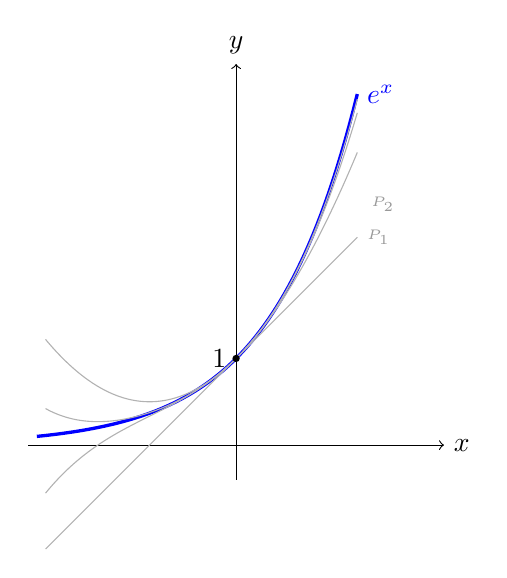
\begin{tikzpicture}[scale=1.1]
\draw[->] (-2.4,0) -- (2.4,0) node[right] {$x$};
\draw[->] (0,-0.4) -- (0,4.4) node[above] {$y$};
% Smooth e^x reference curve
\draw[blue, very thick, domain=-2.3:1.4, samples=80] plot (\x,{exp(\x)});
\node[blue, right] at (1.4,{exp(1.4)}) {$e^{x}$};
% P_1(x) = 1 + x
\draw[gray!60, thin, domain=-2.2:1.4, samples=2] plot (\x,{1 + \x});
\node[gray!80, right] at (1.4,2.4) {\tiny $P_{1}$};
% P_2(x) = 1 + x + x^2/2
\draw[gray!60, thin, domain=-2.2:1.4, samples=80] plot (\x,{1 + \x + \x*\x/2});
\node[gray!80, right] at (1.45,2.78) {\tiny $P_{2}$};
% P_3(x) = 1 + x + x^2/2 + x^3/6
\draw[gray!60, thin, domain=-2.2:1.4, samples=80] plot (\x,{1 + \x + \x*\x/2 + \x*\x*\x/6});
% P_4(x)
\draw[gray!60, thin, domain=-2.2:1.4, samples=80] plot (\x,{1 + \x + \x*\x/2 + \x*\x*\x/6 + \x*\x*\x*\x/24});
% Mark axes
\node[left] at (0,1) {$1$};
\fill (0,1) circle (1.2pt);
\end{tikzpicture}
\caption{The partial sums \(P_{k}(x) = \sum_{n = 0}^{k} x^{n}/n!\) for \(k = 1, 2, 3, 4\) (gray) approach the smooth exponential curve \(e^{x}\) (blue). For \(\lvert x \rvert\) bounded, the convergence is rapid; the tail bound in the proof of \cref{thm:exp-series-converges-positive} quantifies the rate.}
\label{fig:exp-partial-sums}
\end{figure}

% expansion:summary — closing synthesis paragraph linking to §4.2
\Cref{thm:exp-series-converges-positive} establishes that \(e^{x}\) is well defined for \(x > 0\), and direct evaluation shows \(e^{0} = 1\). The case \(x < 0\) is more delicate: the series alternates in sign and is not non-decreasing, so \cref{thm:completeness} alone does not deliver convergence. A different tool --- the result that a series of terms whose absolute values converge is itself convergent --- handles that case, and the same machinery delivers the continuity of \(e^{x}\) and the exponent law. The next section assembles both.

\section{Continuity and the Exponent Law for \texorpdfstring{$e^{x}$}{e\^{}x}}\label{sec:continuity-and-exponent-law}

% expansion:intuition — section opener pivoting from §4.1's three open questions: x < 0 convergence, continuity, exponent law
\Cref{sec:construction-of-exp} defined \(e^{x}\) by its power series and proved the series converges for \(x > 0\). Three claims remain: that the series converges for \(x < 0\) (where the alternating signs prevent the simple tail-bound argument), that \(e^{x}\) is continuous on all of \(\mathbb{R}\), and that \(e^{x} e^{y} = e^{x + y}\) holds for every pair of real numbers \(x, y\). All three follow from a more flexible convergence tool --- absolute convergence implies convergence --- and a careful series-multiplication argument. The exponent law, in particular, requires multiplying out two infinite series and matching the result against the series for \(e^{x + y}\), which is where most of the technical work of this section sits.

\subsection{Continuity of \texorpdfstring{$e^{x}$}{e\^{}x} on the positive reals}

The continuity of \(e^{x}\) at a positive base point \(x_{0}\) is proved by approximating \(e^{x}\) and \(e^{x_{0}}\) by the same partial-sum polynomial \(P_{k}(x) = \sum_{n = 0}^{k} x^{n}/n!\), then using the continuity of \(P_{k}\) (every polynomial is continuous, by \cref{prop:polynomial-limit}) to control the remaining error.

\begin{theorem}\label{thm:exp-continuous-positive}\index{exponential function!continuity}
The function \(e^{x}\) is continuous at every \(x_{0} > 0\): \(\lim_{x \to x_{0}} e^{x} = e^{x_{0}}\).
\end{theorem}

\begin{proof}
Let \(P_{k}(x) = \sum_{n = 0}^{k} x^{n}/n!\) be the \(k\)-th partial sum. From the proof of \cref{thm:exp-series-converges-positive}, for any \(L > 0\), \(0 < x < L\), and \(k > n_{0} > 2L\),
\[
0 \leq e^{x} - P_{k}(x) \leq \frac{x^{n_{0}}}{n_{0}!} \cdot \left(\frac{1}{2}\right)^{k - n_{0}} \leq \frac{L^{n_{0}}}{n_{0}!} \cdot \left(\frac{1}{2}\right)^{k - n_{0}}.
\]
Given \(\varepsilon > 0\), choose \(L = x_{0} + 1\) (so \(0 < x_{0} < L\)) and pick \(k > n_{0} > 2(x_{0} + 1)\) large enough that
\[
\frac{(x_{0} + 1)^{n_{0}}}{n_{0}!} \left(\frac{1}{2}\right)^{k - n_{0}} < \varepsilon.
\]
The polynomial \(P_{k}(x)\) is continuous, so there is a \(\delta > 0\) (with \(\delta \leq \min\{x_{0}/2, 1/2\}\)) such that
\[
\lvert P_{k}(x) - P_{k}(x_{0}) \rvert < \varepsilon \quad \text{whenever } \lvert x - x_{0} \rvert < \delta.
\]
For \(\lvert x - x_{0} \rvert < \delta\) we then have \(0 < x < x_{0} + 1 = L\), so the tail bound applies to both \(e^{x} - P_{k}(x)\) and \(e^{x_{0}} - P_{k}(x_{0})\). Combining:
\begin{aligneddisplay}
\lvert e^{x} - e^{x_{0}} \rvert
&\leq \lvert e^{x} - P_{k}(x) \rvert + \lvert P_{k}(x) - P_{k}(x_{0}) \rvert + \lvert P_{k}(x_{0}) - e^{x_{0}} \rvert \\
&< \varepsilon + \varepsilon + \varepsilon = 3 \varepsilon.
\end{aligneddisplay}
Since \(\varepsilon > 0\) was arbitrary, \(\lim_{x \to x_{0}} e^{x} = e^{x_{0}}\).
\end{proof}

% expansion:intuition — explicitly name the technique used in the proof; it'll reappear throughout the chapter
\begin{remark}[The polynomial-approximation technique]
The proof above is the workhorse of this chapter: approximate \(e^{x}\) and \(e^{x_{0}}\) by a single polynomial \(P_{k}\) chosen so the tail errors are small, then use the continuity of \(P_{k}\) to bound the polynomial difference. Every continuity-style claim in \cref{sec:continuity-and-exponent-law} (and the derivative argument in \cref{sec:rigorous-derivative-of-exp}) follows the same template. The cost is a little bookkeeping (track three error pieces); the payoff is rigour without circularity.
\end{remark}

\subsection{Cauchy sequences and absolute convergence}

To extend the series convergence to \(x < 0\), where the terms alternate in sign and the partial sums are not monotone, we need a tool that allows convergence to be deduced from a property of the absolute values of the terms. The relevant property is \emph{absolute convergence}.

\begin{definition}\label{def:cauchy-sequence}\index{Cauchy sequence}\index{sequence!Cauchy}
A sequence \(\{a_{n}\}_{n = 1}^{\infty}\) of real numbers is a \emph{Cauchy sequence} if for every \(\varepsilon > 0\), there exists \(N_{0} \in \mathbb{N}\) such that
\[
\lvert a_{m} - a_{n} \rvert < \varepsilon \quad \text{for all } m, n \geq N_{0}.
\]

% expansion:intuition — Informally gloss
\emph{Informally, a Cauchy sequence is one whose terms eventually all lie within an arbitrarily small window of each other --- the sequence's tail bunches up. Convergence requires the tail to bunch up around a specific real number; the Cauchy condition asks for the bunching alone, without naming the limit.}
\end{definition}

\begin{theorem}\label{thm:cauchy-iff-convergent}\index{Cauchy sequence!equivalence with convergence}
A sequence of real numbers is convergent if and only if it is a Cauchy sequence.
\end{theorem}

The proof of \cref{thm:cauchy-iff-convergent} requires more setup than \cref{thm:completeness}: the easy direction (convergent \(\Rightarrow\) Cauchy) is a quick triangle-inequality argument, but the reverse direction (Cauchy \(\Rightarrow\) convergent) needs to manufacture a limit out of a sequence that is only known to be self-consistent. We extract the limit through a convergent subsequence, which exists by the Bolzano--Weierstrass theorem; the latter rests on a clever combinatorial fact about monotone subsequences.

\begin{proof}[Proof of \cref{thm:cauchy-iff-convergent}, \(\Rightarrow\) direction]
Suppose \(a_{n} \to L\). Given \(\varepsilon > 0\), pick \(N\) such that \(\lvert a_{n} - L \rvert < \varepsilon / 2\) for all \(n \geq N\). Then for \(m, n \geq N\),
\[
\lvert a_{m} - a_{n} \rvert
= \lvert (a_{m} - L) - (a_{n} - L) \rvert
\leq \lvert a_{m} - L \rvert + \lvert a_{n} - L \rvert
< \frac{\varepsilon}{2} + \frac{\varepsilon}{2}
= \varepsilon.
\]
Hence \(\{a_{n}\}\) is Cauchy.
\end{proof}

The reverse direction is harder. We pick up two lemmas first.

\begin{lemma}\label{lem:cauchy-bounded}
A Cauchy sequence is bounded.
\end{lemma}

\begin{proof}
Let \(\{a_{n}\}\) be Cauchy. Apply the Cauchy condition with \(\varepsilon = 1\) to get an index \(N_{0}\) such that \(\lvert a_{m} - a_{N_{0}} \rvert < 1\) for all \(m \geq N_{0}\). Then \(\lvert a_{m} \rvert \leq \lvert a_{N_{0}} \rvert + 1\) for \(m \geq N_{0}\). Setting
\[
M = \max\bigl\{\lvert a_{1} \rvert, \lvert a_{2} \rvert, \dots, \lvert a_{N_{0} - 1} \rvert, \lvert a_{N_{0}} \rvert + 1\bigr\},
\]
we have \(\lvert a_{n} \rvert \leq M\) for every \(n \geq 1\).
\end{proof}

\begin{lemma}[Monotone subsequence]\label{lem:monotone-subsequence}
Every sequence of real numbers has a monotone (non-decreasing or non-increasing) subsequence.
\end{lemma}

\begin{proof}
Call an index \(n\) a \emph{peak} of the sequence \(\{a_{n}\}\) if \(a_{n} \geq a_{m}\) for every \(m > n\). Two cases.

\emph{Case 1: there are infinitely many peaks.} List them in order: \(n_{1} < n_{2} < n_{3} < \dots\). For each \(k\), \(n_{k}\) is a peak, so \(a_{n_{k}} \geq a_{m}\) for every \(m > n_{k}\); in particular \(a_{n_{k}} \geq a_{n_{k + 1}}\). The subsequence \(\{a_{n_{k}}\}\) is non-increasing.

\emph{Case 2: there are finitely many peaks.} Let \(N\) be greater than the index of every peak. Then no \(n > N\) is a peak, which means: for every \(n > N\) there exists \(m > n\) with \(a_{m} > a_{n}\). Build a subsequence by setting \(n_{1} = N + 1\) and recursively choosing \(n_{k + 1} > n_{k}\) with \(a_{n_{k + 1}} > a_{n_{k}}\). The subsequence \(\{a_{n_{k}}\}\) is strictly increasing, hence non-decreasing.
\end{proof}

\begin{theorem}[Bolzano--Weierstrass]\label{thm:bolzano-weierstrass}\index{Bolzano--Weierstrass theorem}\index{Bolzano--Weierstrass}
Every bounded sequence of real numbers has a convergent subsequence.
\end{theorem}

\begin{proof}
By \cref{lem:monotone-subsequence}, the sequence has a monotone subsequence; the subsequence is bounded (any subsequence of a bounded sequence is bounded). A bounded monotone sequence converges by \cref{thm:completeness}.
\end{proof}

\begin{proof}[Proof of \cref{thm:cauchy-iff-convergent}, \(\Leftarrow\) direction]
Let \(\{a_{n}\}\) be Cauchy. By \cref{lem:cauchy-bounded} it is bounded; by \cref{thm:bolzano-weierstrass} it has a convergent subsequence \(\{a_{n_{k}}\}\) with limit \(L\) for some \(L \in \mathbb{R}\). We claim the full sequence converges to \(L\).

Given \(\varepsilon > 0\), apply the Cauchy condition to find \(N_{1}\) such that \(\lvert a_{m} - a_{n} \rvert < \varepsilon / 2\) for all \(m, n \geq N_{1}\). Apply the subsequence convergence to find \(K\) such that \(\lvert a_{n_{K}} - L \rvert < \varepsilon / 2\) and \(n_{K} \geq N_{1}\) (the second condition is automatic for \(K\) large enough since \(n_{K} \to \infty\)). Then for every \(n \geq N_{1}\),
\[
\lvert a_{n} - L \rvert
\leq \lvert a_{n} - a_{n_{K}} \rvert + \lvert a_{n_{K}} - L \rvert
< \frac{\varepsilon}{2} + \frac{\varepsilon}{2}
= \varepsilon,
\]
where the first term is bounded by the Cauchy condition (since both \(n\) and \(n_{K}\) are at least \(N_{1}\)). Hence \(a_{n} \to L\).
\end{proof}

% expansion:caution — flag the dependency on Bolzano-Weierstrass and the completeness theorem
\begin{caution}
The reverse direction of \cref{thm:cauchy-iff-convergent} depends on \cref{thm:bolzano-weierstrass}, which in turn rests on the monotone-bounded form of completeness (\cref{thm:completeness}). The chain of dependencies makes \cref{thm:cauchy-iff-convergent} ``logically equivalent'' to completeness: any complete ordered field has the Cauchy criterion, and conversely. We will use the theorem freely from this point on, the way \cref{thm:completeness} itself is used.
\end{caution}

The next proposition is the bridge between absolute and ordinary convergence; it is the tool that lets us extend \(e^{x}\) from \(x > 0\) to all of \(\mathbb{R}\).

\begin{proposition}[Absolute convergence implies convergence]\label{prop:abs-conv-implies-conv}\index{convergence!absolute}\index{series!absolute convergence}
Suppose \(\{a_{n}\}_{n = 1}^{\infty}\) is a sequence of real numbers with \(\sum_{n = 1}^{\infty} \lvert a_{n} \rvert < \infty\). Then \(\sum_{n = 1}^{\infty} a_{n}\) converges.
\end{proposition}

\begin{proof}
Let \(S_{n} = \sum_{k = 1}^{n} a_{k}\) be the partial sums of the original series, and \(T_{n} = \sum_{k = 1}^{n} \lvert a_{k} \rvert\) the partial sums of the absolute series. By assumption \(\{T_{n}\}\) converges (it is non-decreasing and bounded, so \cref{thm:completeness} gives the limit). A convergent sequence is Cauchy, so for every \(\varepsilon > 0\) there is some \(N_{0}\) with \(\lvert T_{m} - T_{n} \rvert < \varepsilon\) for all \(m, n \geq N_{0}\). Then for \(m > n \geq N_{0}\),
\[
\lvert S_{m} - S_{n} \rvert
= \left\lvert \sum_{k = n + 1}^{m} a_{k} \right\rvert
\leq \sum_{k = n + 1}^{m} \lvert a_{k} \rvert
= T_{m} - T_{n}
< \varepsilon.
\]
Hence \(\{S_{n}\}\) is also Cauchy, and by \cref{thm:cauchy-iff-convergent} it converges.
\end{proof}

\subsection{Convergence of \texorpdfstring{$e^{x}$}{e\^{}x} for negative \texorpdfstring{$x$}{x}}

For \(x < 0\), set \(y = -x > 0\). The series \(\sum y^{n}/n!\) converges by \cref{thm:exp-series-converges-positive}, so \(\sum \lvert x^{n}/n! \rvert = \sum y^{n}/n!\) is finite. By \cref{prop:abs-conv-implies-conv}, the series \(\sum x^{n}/n!\) itself converges. Combined with \cref{thm:exp-series-converges-positive} for \(x > 0\) and direct evaluation at \(x = 0\):

\begin{corollary}\label{cor:exp-defined-on-R}
The series \(\sum_{n = 0}^{\infty} x^{n}/n!\) converges to a finite real number for every \(x \in \mathbb{R}\); the function \(e^{x}\) is therefore defined on all of \(\mathbb{R}\).
\end{corollary}

The continuity proof from \cref{thm:exp-continuous-positive} also extends: the same polynomial-approximation argument works for \(x_{0} \leq 0\) once the tail bound is replaced by an absolute-value version.

\begin{theorem}\label{thm:exp-continuous}\index{exponential function!continuity (full)}
The function \(e^{x}\) is continuous at every \(x_{0} \in \mathbb{R}\).
\end{theorem}

\begin{proof}[Sketch]
For \(x_{0} > 0\) the proof of \cref{thm:exp-continuous-positive} applies directly. For \(x_{0} \leq 0\), pick \(L\) with \(\lvert x_{0} \rvert < L\), and observe that for \(\lvert x \rvert < L\) and \(k > n_{0} > 2L\),
\[
\left\lvert e^{x} - P_{k}(x) \right\rvert \leq \sum_{n = k + 1}^{\infty} \frac{\lvert x \rvert^{n}}{n!} \leq \frac{L^{n_{0}}}{n_{0}!} \left(\frac{1}{2}\right)^{k - n_{0}}
\]
by the same geometric-tail argument as \cref{thm:exp-series-converges-positive} but applied to \(\sum \lvert x \rvert^{n}/n!\). The three-term decomposition of the proof of \cref{thm:exp-continuous-positive} then proceeds unchanged.
\end{proof}

\subsection{The exponent law}

The most important algebraic property of \(e^{x}\) --- and the source of its name --- is that multiplication of exponentials corresponds to addition of exponents.

\begin{theorem}[Exponent law]\label{thm:exponent-law}\index{exponent law}\index{exponential function!exponent law}
For every \(x, y \in \mathbb{R}\),
\[
e^{x} e^{y} = e^{x + y}.
\]
\end{theorem}

\begin{proof}
Fix \(L > 0\) and assume \(x, y \in [-L, L]\); the result for arbitrary real \(x, y\) follows by taking \(L\) large enough. Pick \(n_{0} \in \mathbb{N}\) with \(n_{0} > 8 L\), and consider partial-sum truncations \(P_{k}(x) = \sum_{n = 0}^{k} x^{n}/n!\) for \(k > n_{0}\).

\emph{Step 1: expand and split the product of partial sums.} Multiplying out,
\[
P_{k}(x) \cdot P_{k}(y) = \left(\sum_{m = 0}^{k} \frac{x^{m}}{m!}\right) \left(\sum_{n = 0}^{k} \frac{y^{n}}{n!}\right)
= \sum_{m = 0}^{k} \sum_{n = 0}^{k} \frac{x^{m} y^{n}}{m! \, n!}.
\]
Reorganise the double sum by total exponent \(\ell = m + n\). The pair \((m, n)\) with \(m, n \in \{0, 1, \dots, k\}\) and \(m + n = \ell\) ranges over \(0 \leq \ell \leq 2k\). For \(\ell \leq k\), \(m\) ranges over \(\{0, 1, \dots, \ell\}\); for \(\ell > k\) (i.e., \(\ell = k + j\) with \(j \in \{1, \dots, k\}\)), the constraint \(n = \ell - m \leq k\) forces \(m \geq j\), and \(m \leq k\) is automatic, so \(m\) ranges over \(\{j, j + 1, \dots, k\}\). Therefore
\[
P_{k}(x) \cdot P_{k}(y)
= \underbrace{\sum_{\ell = 0}^{k} \sum_{m = 0}^{\ell} \frac{x^{m} y^{\ell - m}}{m! (\ell - m)!}}_{\text{(I)}}
+ \underbrace{\sum_{j = 1}^{k} \sum_{m = j}^{k} \frac{x^{m} y^{k + j - m}}{m! (k + j - m)!}}_{\text{(II)}}.
\]

\emph{Step 2: piece (I) equals \(P_{k}(x + y)\).} Pull out a factor of \(1/\ell!\) and use the binomial theorem \((x + y)^{\ell} = \sum_{m = 0}^{\ell} \binom{\ell}{m} x^{m} y^{\ell - m}\):
\begin{aligneddisplay}
\text{(I)}
&= \sum_{\ell = 0}^{k} \frac{1}{\ell!} \sum_{m = 0}^{\ell} \frac{\ell!}{m! (\ell - m)!} x^{m} y^{\ell - m} \\
&= \sum_{\ell = 0}^{k} \frac{1}{\ell!} \sum_{m = 0}^{\ell} \binom{\ell}{m} x^{m} y^{\ell - m} \\
&= \sum_{\ell = 0}^{k} \frac{(x + y)^{\ell}}{\ell!}
 = P_{k}(x + y).
\end{aligneddisplay}

\emph{Step 3: bound piece (II).} Take absolute values and reindex. Each term in (II) has \(m + (k + j - m) = k + j\), so the total exponent ranges over \(\{k + 1, \dots, 2k\}\). Write \(\ell = k + j\); then for fixed \(\ell\) the inner sum runs over \(m \in \{\ell - k, \dots, k\}\), which is a subset of \(\{0, 1, \dots, \ell\}\). Therefore
\begin{aligneddisplay}
\lvert \text{(II)} \rvert
&\leq \sum_{j = 1}^{k} \sum_{m = j}^{k} \frac{\lvert x \rvert^{m} \lvert y \rvert^{k + j - m}}{m! (k + j - m)!} \\
&\leq \sum_{\ell = k + 1}^{2k} \sum_{m = 0}^{\ell} \frac{\lvert x \rvert^{m} \lvert y \rvert^{\ell - m}}{m! (\ell - m)!} \\
&= \sum_{\ell = k + 1}^{2k} \frac{(\lvert x \rvert + \lvert y \rvert)^{\ell}}{\ell!}
\leq \sum_{\ell = k + 1}^{2k} \frac{(2L)^{\ell}}{\ell!},
\end{aligneddisplay}
where the second inequality enlarges the index set (the missing terms with \(m \notin \{\ell - k, \dots, k\}\) are non-negative), the equality reverses Step 2 with \(\lvert x \rvert\) and \(\lvert y \rvert\) in place of \(x\) and \(y\), and the last inequality uses \(\lvert x \rvert + \lvert y \rvert \leq 2L\).

For \(n_{0} > 8 L\) we have \((2L)/(n_{0} + 1) < 1/4 < 1/2\), so the geometric-tail argument from \cref{thm:exp-series-converges-positive} applied to \(\sum (2L)^{\ell}/\ell!\) gives
\[
\sum_{\ell = k + 1}^{2k} \frac{(2L)^{\ell}}{\ell!}
\leq \sum_{\ell = n_{0} + 1}^{\infty} \frac{(2L)^{\ell}}{\ell!}
\leq \frac{(2L)^{n_{0}}}{n_{0}!} \cdot \left(\frac{1}{2}\right)^{k - n_{0}}
\quad \text{for } k > n_{0}.
\]
Combining steps 2 and 3,
\[
\bigl\lvert P_{k}(x) P_{k}(y) - P_{k}(x + y) \bigr\rvert = \lvert \text{(II)} \rvert \leq \frac{(2L)^{n_{0}}}{n_{0}!} \cdot \left(\frac{1}{2}\right)^{k - n_{0}}. \tag{\(*\)}
\]

\emph{Step 4: bound \(\lvert e^{x} - P_{k}(x) \rvert\) and similarly for \(y\) and \(x + y\).} The proof of \cref{thm:exp-continuous} applied to absolute values gives
\[
\bigl\lvert e^{x} - P_{k}(x) \bigr\rvert \leq \frac{L^{n_{0}}}{n_{0}!} \cdot \left(\frac{1}{2}\right)^{k - n_{0}}
\]
for \(\lvert x \rvert \leq L\), and analogously for \(y\). For \(x + y\), \(\lvert x + y \rvert \leq 2 L\), so the same template gives
\[
\bigl\lvert e^{x + y} - P_{k}(x + y) \bigr\rvert \leq \frac{(2L)^{n_{0}}}{n_{0}!} \cdot \left(\frac{1}{2}\right)^{k - n_{0}}. \tag{\(**\)}
\]

\emph{Step 5: combine the bounds.} Telescope the difference:
\begin{aligneddisplay}
e^{x} e^{y} - e^{x + y}
&= \bigl(e^{x} - P_{k}(x)\bigr) e^{y} + P_{k}(x) \bigl(e^{y} - P_{k}(y)\bigr) \\
&\quad + \bigl(P_{k}(x) P_{k}(y) - P_{k}(x + y)\bigr) + \bigl(P_{k}(x + y) - e^{x + y}\bigr).
\end{aligneddisplay}
Use the absolute-value bound
\[
\lvert e^{y} \rvert = \left\lvert \sum_{n = 0}^{\infty} \frac{y^{n}}{n!} \right\rvert
\leq \sum_{n = 0}^{\infty} \frac{\lvert y \rvert^{n}}{n!}
= e^{\lvert y \rvert}
\leq e^{L},
\]
where the last inequality uses \(\lvert y \rvert \leq L\) and the term-by-term monotonicity \(0 \leq |y| \leq L \Rightarrow |y|^{n} \leq L^{n}\) for every \(n \geq 0\). The same argument applied to the partial sum gives \(\lvert P_{k}(x) \rvert \leq P_{k}(\lvert x \rvert) \leq e^{L}\). Then by the bounds above,
\begin{aligneddisplay}
\bigl\lvert e^{x} e^{y} - e^{x + y} \bigr\rvert
&\leq \bigl\lvert e^{x} - P_{k}(x) \bigr\rvert \cdot e^{L}
+ e^{L} \cdot \bigl\lvert e^{y} - P_{k}(y) \bigr\rvert \\
&\quad + \bigl\lvert P_{k}(x) P_{k}(y) - P_{k}(x + y) \bigr\rvert
+ \bigl\lvert P_{k}(x + y) - e^{x + y} \bigr\rvert \\
&\leq \frac{L^{n_{0}}}{n_{0}!} \left(\frac{1}{2}\right)^{k - n_{0}} \cdot e^{L}
+ e^{L} \cdot \frac{L^{n_{0}}}{n_{0}!} \left(\frac{1}{2}\right)^{k - n_{0}} \\
&\quad + \frac{(2L)^{n_{0}}}{n_{0}!} \left(\frac{1}{2}\right)^{k - n_{0}}
+ \frac{(2L)^{n_{0}}}{n_{0}!} \left(\frac{1}{2}\right)^{k - n_{0}} \\
&= \left[\frac{2 e^{L} L^{n_{0}} + 2 (2L)^{n_{0}}}{n_{0}!}\right] \cdot \left(\frac{1}{2}\right)^{k - n_{0}}.
\end{aligneddisplay}
The bracket is a fixed constant (independent of \(k\)), and \((1/2)^{k - n_{0}} \to 0\) as \(k \to \infty\). Therefore the right-hand side goes to \(0\), and since the left-hand side is independent of \(k\),
\[
\bigl\lvert e^{x} e^{y} - e^{x + y} \bigr\rvert = 0,
\]
i.e., \(e^{x} e^{y} = e^{x + y}\) for every \(x, y \in [-L, L]\).

\emph{Step 6: extend to all of \(\mathbb{R}\).} For arbitrary \(x, y \in \mathbb{R}\), pick \(L > 0\) large enough that \(\lvert x \rvert, \lvert y \rvert \leq L\) (e.g., \(L = \max\{\lvert x \rvert, \lvert y \rvert\} + 1\)). Step 5 then gives \(e^{x} e^{y} = e^{x + y}\). Since \(L\) was arbitrary, the identity holds for every pair of real numbers.
\end{proof}

% expansion:caution — the proof outline summarizes a lot of bookkeeping; flag the load-bearing facts
\begin{caution}
The proof of \cref{thm:exponent-law} is the most computationally heavy result in the chapter, and it relies on three tools we have already developed: the partial-sum machinery from \cref{sec:construction-of-exp}, the binomial theorem (used implicitly when collecting coefficients of \(x^{m} y^{n}\) with fixed sum), and \cref{thm:exp-continuous} (to take the limit of products through the partial sums). Each is doing real work; if any failed, the exponent law would too. The result itself is the algebraic backbone of every later property of \(e^{x}\) --- including the strict-monotonicity argument in \cref{sec:logarithm} that makes \(\ln x\) well defined.
\end{caution}

\begin{workedexample}
\begin{example}\label{ex:exponent-law-numerical}
Verify the exponent law numerically at \(x = 1\), \(y = 1\): compare \(e^{1} \cdot e^{1}\) and \(e^{2}\).
\end{example}

\begin{solution}
From \cref{ex:partial-sum-e}, \(e^{1} \approx 2.71828\), so \(e^{1} \cdot e^{1} \approx (2.71828)^{2} \approx 7.38906\). Direct evaluation of the series for \(e^{2}\):
\[
e^{2} = 1 + 2 + 2 + \frac{4}{3} + \frac{2}{3} + \frac{4}{15} + \dots \approx 7.38906,
\]
matching to all four decimal places. \cref{thm:exponent-law} guarantees that the agreement is exact (modulo the truncation error in the partial-sum approximations).
\end{solution}
\end{workedexample}

% expansion:summary — closing synthesis paragraph linking to §4.3
With \(e^{x}\) defined on \(\mathbb{R}\), continuous, and satisfying the exponent law, every claim about the exponential made informally in earlier chapters is now a theorem. The remaining piece is the derivative: Chapter 2 proved \((e^{x})' = e^{x}\) by a casual term-by-term argument that took the convergence and continuity for granted. The next section re-derives the derivative rigorously, this time with an explicit error bound on \((e^{h} - 1)/h - 1\) that locks the limit at \(1\) without circularity.

\section{The Derivative of \texorpdfstring{$e^{x}$}{e\^{}x}}\label{sec:rigorous-derivative-of-exp}

% expansion:intuition — section opener pivoting from §4.2's preview
\Cref{thm:derivative-of-exp} (Chapter 2) asserted that \((e^{x})' = e^{x}\) and gave a quick term-by-term argument: feed the series into the difference quotient and observe that all but the leading term vanish as \(h \to 0\). The argument was correct in spirit but assumed three properties of \(e^{x}\) that we have only just proved (convergence, continuity, the exponent law). With those in hand, this section re-establishes the derivative formula with an explicit bound that shows exactly how fast \((e^{h} - 1)/h\) approaches \(1\).

\subsection{The bound on \texorpdfstring{$(e^{h} - 1)/h$}{(eh - 1)/h}}

The exponent law lets us factor \(e^{x + h}\) as \(e^{x} \cdot e^{h}\), so the difference quotient becomes
\[
\frac{e^{x + h} - e^{x}}{h} = \frac{e^{x} \cdot e^{h} - e^{x}}{h} = e^{x} \cdot \frac{e^{h} - 1}{h}.
\]
The factor \(e^{x}\) is independent of \(h\); the entire derivative calculation reduces to evaluating \(\lim_{h \to 0} (e^{h} - 1)/h\). We do this directly from the series.

\begin{lemma}\label{lem:eh-minus-1-over-h-bound}
For \(\lvert h \rvert \leq 1/2\),
\[
\left\lvert \frac{e^{h} - 1}{h} - 1 \right\rvert \leq \lvert h \rvert.
\]
In particular \(\lim_{h \to 0} (e^{h} - 1)/h = 1\).
\end{lemma}

\begin{proof}
By the series definition (\cref{def:exponential-function}),
\[
e^{h} - 1 = h + \frac{h^{2}}{2!} + \frac{h^{3}}{3!} + \dotsb,
\]
so dividing by \(h\) (for \(h \neq 0\)),
\[
\frac{e^{h} - 1}{h} = 1 + \frac{h}{2!} + \frac{h^{2}}{3!} + \frac{h^{3}}{4!} + \dotsb.
\]
The error from \(1\) is therefore
\[
\frac{e^{h} - 1}{h} - 1 = \frac{h}{2!} + \frac{h^{2}}{3!} + \frac{h^{3}}{4!} + \dotsb = h \cdot \left(\frac{1}{2!} + \frac{h}{3!} + \frac{h^{2}}{4!} + \dotsb\right).
\]
Bounding the parenthesised series by absolute values,
\begin{aligneddisplay}
\left\lvert \frac{1}{2!} + \frac{h}{3!} + \frac{h^{2}}{4!} + \dotsb \right\rvert
&\leq \frac{1}{2!} + \frac{\lvert h \rvert}{3!} + \frac{\lvert h \rvert^{2}}{4!} + \dotsb \\
&\leq \frac{1}{2} + \frac{\lvert h \rvert}{6} + \frac{\lvert h \rvert^{2}}{24} + \dotsb \\
&\leq \frac{1}{2} \cdot \left(1 + \lvert h \rvert + \lvert h \rvert^{2} + \dotsb\right)
 = \frac{1}{2} \cdot \frac{1}{1 - \lvert h \rvert},
\end{aligneddisplay}
where we used \(1/n! \leq 1/2\) for every \(n \geq 2\) (since \(n! \geq 2\)) and the geometric-series formula \(1/(1 - r)\) for \(\lvert r \rvert < 1\). For \(\lvert h \rvert \leq 1/2\), \(1/(1 - \lvert h \rvert) \leq 2\), so the parenthesised series is bounded by \(1/2 \cdot 2 = 1\). Therefore
\[
\left\lvert \frac{e^{h} - 1}{h} - 1 \right\rvert \leq \lvert h \rvert \cdot 1 = \lvert h \rvert. \qedhere
\]
\end{proof}

% expansion:caution — comparison to ch02's informal derivation
\begin{caution}
\Cref{lem:eh-minus-1-over-h-bound} is the rigorous version of the term-by-term argument in \cref{thm:derivative-of-exp} (Chapter 2). The earlier proof asserted that all higher-order terms ``vanish as \(h \to 0\)'' without quantifying the rate; the lemma here gives the explicit bound \(\lvert h \rvert\), so the convergence is not just qualitative but proceeds at a rate at least linear in \(h\). For most calculus purposes the qualitative version is enough; for any later argument that needs to track derivative errors quantitatively (Taylor remainders, error analysis), the bound is what we will use.
\end{caution}

\subsection{The derivative formula}

\begin{theorem}\label{thm:exp-derivative-rigorous}\index{exponential function!derivative (rigorous)}
For every \(x \in \mathbb{R}\),
\[
\frac{d}{dx} e^{x} = e^{x}.
\]
\end{theorem}

\begin{proof}
By the exponent law (\cref{thm:exponent-law}) and \cref{lem:eh-minus-1-over-h-bound},
\[
\lim_{h \to 0} \frac{e^{x + h} - e^{x}}{h}
= \lim_{h \to 0} e^{x} \cdot \frac{e^{h} - 1}{h}
= e^{x} \cdot 1
= e^{x},
\]
where the constant \(e^{x}\) was pulled out of the limit. \cref{def:derivative-function} then gives \(\frac{d}{dx} e^{x} = e^{x}\).
\end{proof}

\begin{corollary}\label{cor:exp-higher-derivatives}
Every higher derivative of \(e^{x}\) is itself \(e^{x}\): for every positive integer \(n\), \((e^{x})^{(n)} = e^{x}\).
\end{corollary}

\begin{proof}
Iterate \cref{thm:exp-derivative-rigorous}: \((e^{x})' = e^{x}\), so \((e^{x})'' = (e^{x})' = e^{x}\), and inductively \((e^{x})^{(n)} = e^{x}\).
\end{proof}

% expansion:summary — closing synthesis paragraph linking to §4.4
The exponential function is now fully grounded: defined by a series, continuous, satisfying the exponent law, and with derivative equal to itself. The next missing piece is the logarithm \(\ln x\), which Chapter 3 used informally as the inverse of \(e^{x}\). To construct \(\ln x\) rigorously we need to know that \(e^{x}\) is strictly increasing (so its inverse is well defined). Strict monotonicity is a derivative-driven property --- a function whose derivative is positive is increasing --- and the existence theorem that turns ``derivative positive'' into ``function increasing'' is the Mean Value Theorem. The next section establishes Rolle's theorem and the MVT; the section after applies them to construct \(\ln x\).

\section{Rolle's Theorem and the Mean Value Theorem}\label{sec:rolle-and-mvt}

% expansion:intuition — section opener pivoting from §4.3's preview
The Mean Value Theorem is the central existence theorem of differential calculus. It says that on any closed interval where a function is continuous and differentiable in the interior, there is some point where the instantaneous slope (the derivative) equals the average slope over the interval (the secant slope). This single statement underpins the monotonicity argument we need for \cref{sec:logarithm}, and will reappear constantly in later chapters when we extract qualitative information about a function from quantitative information about its derivative. We approach the MVT in two steps: first \emph{Rolle's theorem}, the special case where the average slope is \(0\), and then the MVT itself, derived by reducing the general case to Rolle's via a simple auxiliary function.

\subsection{Maxima, minima, and Theorem A}

\begin{definition}\label{def:max-min}\index{maximum}\index{minimum}
Let \(f\) be a function defined on a domain \(D \subseteq \mathbb{R}\), and let \(x_{0} \in D\). We say
\begin{itemize}
    \item \(x_{0}\) is a \emph{maximum point} of \(f\) on \(D\) (and \(f(x_{0})\) is the \emph{maximum value}) if \(f(x_{0}) \geq f(x)\) for every \(x \in D\);
    \item \(x_{0}\) is a \emph{minimum point} of \(f\) on \(D\) (and \(f(x_{0})\) is the \emph{minimum value}) if \(f(x_{0}) \leq f(x)\) for every \(x \in D\).
\end{itemize}

% expansion:intuition — Informally gloss
\emph{Informally, a maximum point is where \(f\) attains its largest value on \(D\), and a minimum point is where it attains its smallest. A function may have multiple maximum points (all attaining the same maximum value) or none (if \(D\) is unbounded or open and \(f\) escapes to \(\pm\infty\)).}
\end{definition}

\begin{example}
The function \(\cos x\) on \(\mathbb{R}\) has \(x_{0} = 0\) (and every \(x_{0} = 2\pi k\) for integer \(k\)) as a maximum point, with maximum value \(1\). It has \(x_{0} = \pi\) (and every \(\pi + 2\pi k\)) as a minimum point with minimum value \(-1\).
\end{example}

A foundational fact from real analysis says that closed intervals are well-behaved with respect to attaining extrema.

\begin{theorem}[Extreme value theorem]\label{thm:evt}\index{extreme value theorem}
If \(f\) is continuous on a closed interval \([a, b]\), then \(f\) attains both a maximum and a minimum on \([a, b]\): there exist \(x_{M}, x_{m} \in [a, b]\) with \(f(x_{M}) \geq f(x) \geq f(x_{m})\) for all \(x \in [a, b]\).
\end{theorem}

\begin{remark}
The proof of \cref{thm:evt} uses the completeness of \(\mathbb{R}\) (\cref{thm:completeness}) and is the kind of analytical argument we have so far avoided. We state the theorem without proof and use it as a black box. Both the closedness of the interval and the continuity of \(f\) are essential: \(f(x) = x\) on the open interval \((0, 1)\) attains no maximum (the supremum is \(1\) but is never reached), and a discontinuous function on \([0, 1]\) like the rationals-indicator can fail to attain its maximum even on a closed interval.
\end{remark}

The next theorem is the differential-calculus content: where the maximum or minimum sits inside the interval (not at an endpoint), the derivative must vanish.

\begin{theorem}[Theorem A]\label{thm:interior-extrema}\index{interior extremum theorem}\index{theorem a}
Suppose \(f\) is defined on \([a, b]\), \(x_{M} \in (a, b)\) is a maximum (or minimum) point of \(f\) on \([a, b]\), and \(f'(x_{M})\) exists. Then \(f'(x_{M}) = 0\).
\end{theorem}

\begin{proof}
Take \(x_{M}\) to be a maximum point (the minimum case is parallel; replace \(\geq\) by \(\leq\)). Then \(f(x_{M}) \geq f(x)\) for every \(x \in [a, b]\), which translates to
\[
f(x_{M} + h) - f(x_{M}) \leq 0
\]
for every \(h\) such that \(x_{M} + h \in [a, b]\). Since \(x_{M}\) is in the open interior \((a, b)\), both small positive and small negative values of \(h\) keep \(x_{M} + h\) inside \([a, b]\).

For \(h > 0\), \((f(x_{M} + h) - f(x_{M}))/h \leq 0\), so the right-hand limit
\[
f'(x_{M}) = \lim_{h \to 0^{+}} \frac{f(x_{M} + h) - f(x_{M})}{h} \leq 0.
\]
For \(h < 0\), \((f(x_{M} + h) - f(x_{M}))/h \geq 0\) (negative-over-negative), so
\[
f'(x_{M}) = \lim_{h \to 0^{-}} \frac{f(x_{M} + h) - f(x_{M})}{h} \geq 0.
\]
Both inequalities hold simultaneously, so \(f'(x_{M}) = 0\).
\end{proof}

% expansion:caution — the "interior" condition is essential; endpoint extrema are not bound by f'=0
\begin{caution}
\Cref{thm:interior-extrema} requires \(x_{M}\) to be in the \emph{open} interior \((a, b)\). At endpoints \(a\) or \(b\), an extremum need not have \(f' = 0\): the function \(f(x) = x\) on \([0, 1]\) attains its minimum at \(x = 0\) and its maximum at \(x = 1\), with \(f'(x) = 1 \neq 0\) at every point. The endpoints have only one-sided derivatives available, and the two-sided ``squeeze'' that forces \(f'(x_{M}) = 0\) does not apply.
\end{caution}

\subsection{Rolle's theorem}

Rolle's theorem combines the extreme value theorem (\cref{thm:evt}) with \cref{thm:interior-extrema}. The idea: if \(f\) starts and ends at the same height, an extremum must occur somewhere in the middle, and that interior extremum has zero derivative.

\begin{theorem}[Rolle's theorem]\label{thm:rolle}\index{Rolle's theorem}
Suppose \(f\) is continuous on \([a, b]\) and differentiable on \((a, b)\), with \(f(a) = f(b)\). Then there exists \(c \in (a, b)\) such that \(f'(c) = 0\).
\end{theorem}

\begin{proof}
By \cref{thm:evt}, \(f\) attains a maximum at some \(x_{M} \in [a, b]\) and a minimum at some \(x_{m} \in [a, b]\), with \(f(x_{m}) \leq f(x) \leq f(x_{M})\) for every \(x \in [a, b]\).

\emph{Case 1: \(f(x_{m}) = f(x_{M})\).} Then \(f(x_{m}) \leq f(x) \leq f(x_{M}) = f(x_{m})\) for all \(x\), so \(f\) is constant on \([a, b]\). Then \(f'(c) = 0\) for every \(c \in (a, b)\); pick any.

\emph{Case 2: \(f(x_{m}) < f(x_{M})\).} Then either \(f(x_{M}) > f(a) = f(b)\) or \(f(x_{m}) < f(a) = f(b)\) (or both). In the first case, \(x_{M}\) cannot be \(a\) or \(b\), so \(x_{M} \in (a, b)\); by \cref{thm:interior-extrema}, \(f'(x_{M}) = 0\), and we set \(c = x_{M}\). In the second case the same argument applies to \(x_{m}\), giving \(f'(x_{m}) = 0\) with \(c = x_{m}\).
\end{proof}

\subsection{The Mean Value Theorem}

The MVT generalises Rolle's theorem: instead of demanding equal endpoint values, we allow any pair of endpoint values and conclude that the derivative somewhere matches the average rate of change.

\begin{theorem}[Mean Value Theorem]\label{thm:mvt}\index{mean value theorem}
Suppose \(f\) is continuous on \([a, b]\) and differentiable on \((a, b)\). Then there exists \(c \in (a, b)\) such that
\[
f'(c) = \frac{f(b) - f(a)}{b - a}.
\]
\end{theorem}

% expansion:figure — the canonical MVT picture showing the parallel secant and tangent
\begin{figure}[H]
\centering
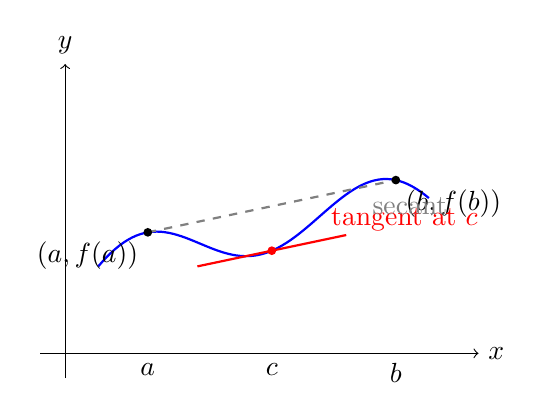
\begin{tikzpicture}[scale=1.05]
\draw[->] (-0.3,0) -- (5,0) node[right] {$x$};
\draw[->] (0,-0.3) -- (0,3.5) node[above] {$y$};
% Curve f(x)
\draw[blue, thick, domain=0.4:4.4, samples=80] plot (\x,{0.5 + 0.7*\x - 0.1*\x*\x + 0.4*sin(2*\x r)});
% Secant line from (a, f(a)) to (b, f(b))
\def\ax{1}
\def\bx{4}
\pgfmathsetmacro{\ay}{0.5 + 0.7*\ax - 0.1*\ax*\ax + 0.4*sin(2*\ax r)}
\pgfmathsetmacro{\by}{0.5 + 0.7*\bx - 0.1*\bx*\bx + 0.4*sin(2*\bx r)}
\draw[gray, dashed, thick] (\ax,\ay) -- (\bx,\by);
\fill (\ax,\ay) circle (1.5pt);
\fill (\bx,\by) circle (1.5pt);
\node[below] at (\ax,0) {$a$};
\node[below] at (\bx,0) {$b$};
\node[below left] at (\ax,\ay) {$(a, f(a))$};
\node[below right] at (\bx,\by) {$(b, f(b))$};
% Compute c (visually, around 2.4-2.6)
\def\cx{2.5}
\pgfmathsetmacro{\cy}{0.5 + 0.7*\cx - 0.1*\cx*\cx + 0.4*sin(2*\cx r)}
\fill[red] (\cx,\cy) circle (1.5pt);
\node[below] at (\cx,0) {$c$};
% Tangent at c (parallel to secant by construction)
\pgfmathsetmacro{\slope}{(\by - \ay)/(\bx - \ax)}
\draw[red, thick] ({\cx-0.9},{\cy - 0.9*\slope}) -- ({\cx+0.9},{\cy + 0.9*\slope});
\node[red, above right] at ({\cx+0.6},{\cy + 0.6*\slope}) {tangent at $c$};
\node[gray, below right] at (3.6,2.0) {secant};
\end{tikzpicture}
\caption{The Mean Value Theorem: the secant line through \((a, f(a))\) and \((b, f(b))\) (dashed) has slope \((f(b) - f(a))/(b - a)\); the MVT guarantees an interior point \(c\) where the tangent (solid) is parallel to the secant.}
\label{fig:mvt}
\end{figure}

\begin{proof}
The strategy is to construct an auxiliary function \(g\) satisfying the hypotheses of Rolle's theorem (\cref{thm:rolle}). Define
\[
g(x) = f(x) - \left[f(a) + \frac{f(b) - f(a)}{b - a}(x - a)\right].
\]
The bracketed expression is the secant line through \((a, f(a))\) and \((b, f(b))\); \(g(x)\) is the vertical gap between the curve \(y = f(x)\) and that secant. By construction:
\begin{itemize}
    \item \(g\) is continuous on \([a, b]\) (sum of continuous functions);
    \item \(g\) is differentiable on \((a, b)\) (sum of differentiable functions);
    \item \(g(a) = f(a) - f(a) = 0\), and \(g(b) = f(b) - f(b) = 0\), so \(g(a) = g(b)\).
\end{itemize}
By Rolle's theorem there exists \(c \in (a, b)\) with \(g'(c) = 0\). Computing,
\[
g'(c) = f'(c) - \frac{f(b) - f(a)}{b - a} = 0,
\]
so \(f'(c) = (f(b) - f(a))/(b - a)\), as required.
\end{proof}

% expansion:caution — hypothesis asymmetry: closed [a,b] for continuity, open (a,b) for differentiability
\begin{caution}
The MVT requires \(f\) to be \emph{continuous on the closed interval \([a, b]\)} and \emph{differentiable on the open interval \((a, b)\)}. Continuity at the endpoints matters because the proof uses the extreme value theorem, which needs a closed interval. Differentiability at the endpoints is \emph{not} required, because Rolle's theorem only invokes the derivative at an interior critical point. A function like \(f(x) = \sqrt{x}\) on \([0, 1]\) is fine (continuous on \([0, 1]\), differentiable on \((0, 1)\) with vertical tangent at \(0\) excluded), and the MVT applies to it.
\end{caution}

% expansion:strategy — the verification routine for applying MVT, since hypothesis-checking is the most common stumble
\begin{strategy}[Applying the MVT]
To use the MVT to extract information about \(f'\) on an interval \([a, b]\):
\begin{enumerate}
    \item Verify that \(f\) is continuous on the closed interval \([a, b]\). Endpoints count.
    \item Verify that \(f\) is differentiable on the open interval \((a, b)\). Endpoints don't count.
    \item Apply the conclusion: \emph{there exists} \(c \in (a, b)\) with \(f'(c) = (f(b) - f(a))/(b - a)\). The MVT guarantees existence; it does not tell us which \(c\), so any subsequent argument must use only the existence, not a specific value.
\end{enumerate}
The most common error is applying the MVT to a function that fails one of the hypotheses; the conclusion can then easily be false. \(\lvert x \rvert\) on \([-1, 1]\) is continuous everywhere but not differentiable at \(0\); the secant slope is \(0\), but no \(c \in (-1, 1)\) has \(\lvert x \rvert' (c) = 0\) (the derivative is \(\pm 1\) where it exists), and the contradiction reveals the missing differentiability hypothesis.
\end{strategy}

% expansion:summary — closing synthesis paragraph linking to §4.5
With Rolle's theorem and the MVT in hand, we can now turn the qualitative claim ``\(f' \geq 0\) means \(f\) is increasing'' into a genuine theorem. The next section establishes the corollary, applies it to show that \(e^{x}\) is strictly increasing, defines \(\ln x\) as the inverse of the now-strictly-increasing exponential, and computes its derivative without any of the circularity worries that haunted Chapter 3.

\section{Monotonicity and the Logarithmic Function}\label{sec:logarithm}

% expansion:intuition — section opener pivoting from §4.4's preview about MVT delivering monotonicity
The Mean Value Theorem of \cref{sec:rolle-and-mvt} converts pointwise information about the derivative into structural information about the function on an interval. The cleanest such conversion is monotonicity: if the derivative is non-negative throughout an interval, the function is non-decreasing on that interval, and if the derivative is strictly positive, the function is strictly increasing. Applied to \(e^{x}\) (whose derivative \(e^{x}\) is positive everywhere), strict monotonicity follows immediately --- and that is exactly what is needed to define the inverse \(\ln x\) cleanly. This section assembles the corollary, defines \(\ln x\) as the inverse of \(e^{x}\), proves the continuity of \(\ln x\) by an argument based on its strict monotonicity, and finally computes \(d/dx \ln x\) rigorously via the inverse-function technique --- closing the loop from \cref{sec:chain-rule-applications}, where this derivative was computed informally.

\subsection{Monotonicity from the sign of the derivative}

\begin{corollary}[Monotonicity from \(f' \geq 0\)]\label{cor:monotonicity}\index{monotonicity}\index{increasing function}
Suppose \(f\) is continuous on \([a, b]\) and differentiable on \((a, b)\).
\begin{itemize}
    \item If \(f'(c) \geq 0\) for every \(c \in (a, b)\), then \(f(x_{1}) \leq f(x_{2})\) for every \(x_{1}, x_{2} \in [a, b]\) with \(x_{1} \leq x_{2}\) (\(f\) is non-decreasing on \([a, b]\)).
    \item If furthermore \(f'(c) > 0\) for every \(c \in (a, b)\), then \(f(x_{1}) < f(x_{2})\) for every \(x_{1}, x_{2} \in [a, b]\) with \(x_{1} < x_{2}\) (\(f\) is strictly increasing on \([a, b]\)).
\end{itemize}
\end{corollary}

\begin{proof}
For \(x_{1}, x_{2} \in [a, b]\) with \(x_{1} < x_{2}\), apply the MVT (\cref{thm:mvt}) on the subinterval \([x_{1}, x_{2}]\). The hypotheses of \cref{thm:mvt} hold on this subinterval (continuity on \([x_{1}, x_{2}] \subseteq [a, b]\), differentiability on \((x_{1}, x_{2}) \subseteq (a, b)\)), so there exists \(c \in (x_{1}, x_{2})\) with
\[
f'(c) = \frac{f(x_{2}) - f(x_{1})}{x_{2} - x_{1}}.
\]
The denominator \(x_{2} - x_{1}\) is positive. If \(f'(c) \geq 0\), the numerator is non-negative, so \(f(x_{2}) \geq f(x_{1})\). If \(f'(c) > 0\), the numerator is strictly positive, so \(f(x_{2}) > f(x_{1})\).
\end{proof}

\begin{example}[Sine on \([0, \pi/4]\)]
The derivative \((\sin x)' = \cos x\) (\cref{thm:derivative-sin}) is positive on \((0, \pi/4) \subseteq (0, \pi/2)\), where cosine is positive. By \cref{cor:monotonicity}, \(\sin\) is strictly increasing on \([0, \pi/4]\): for \(0 \leq x_{1} < x_{2} \leq \pi/4\), \(\sin x_{1} < \sin x_{2}\). The same argument extends \(\sin\) being strictly increasing to \([0, \pi/2]\) where \(\cos\) remains positive.
\end{example}

\begin{example}[Exponential on \(\mathbb{R}\)]\label{ex:exp-strictly-increasing}
The derivative \((e^{x})' = e^{x}\) (\cref{thm:exp-derivative-rigorous}). The series definition gives \(e^{x} > 0\) for every \(x \in \mathbb{R}\) (positive when \(x \geq 0\) by direct inspection; for \(x < 0\), \(e^{x} = 1/e^{-x} > 0\) using the exponent law from \cref{thm:exponent-law}). By \cref{cor:monotonicity}, \(e^{x}\) is strictly increasing on every closed interval, hence strictly increasing on \(\mathbb{R}\).
\end{example}

% expansion:caution — the leap from "strictly increasing on every closed interval" to "strictly increasing on R" deserves a flag
\begin{caution}
\Cref{cor:monotonicity} is stated on a closed interval \([a, b]\), but the conclusion ``strictly increasing on \(\mathbb{R}\)'' for \(e^{x}\) extends because for any \(x_{1} < x_{2}\) in \(\mathbb{R}\) we can apply the corollary on \([x_{1}, x_{2}]\). The same is not true of every interval-bounded result --- some properties (boundedness, attaining a maximum) can fail when the interval is unbounded --- but strict monotonicity is preserved by the obvious argument.
\end{caution}

\subsection{Defining \texorpdfstring{$\ln x$}{ln x}}

\Cref{ex:exp-strictly-increasing} gave us what we need: \(e^{x}\) is strictly increasing on \(\mathbb{R}\). Strict monotonicity is exactly the one-to-one criterion of \cref{def:one-to-one}, so \(e^{x}\) has an inverse function on its range. The range of \(e^{x}\) is \((0, \infty)\) (we will not prove this explicitly; it follows from continuity and the limits \(\lim_{x \to \infty} e^{x} = \infty\) and \(\lim_{x \to -\infty} e^{x} = 0\), which can be derived from the series).

\begin{definition}\label{def:logarithm}\index{logarithm}\index{ln@$\ln x$}\index{natural logarithm}
For \(x \in (0, \infty)\), the \emph{natural logarithm} of \(x\), denoted \(\ln x\), is the unique real number \(a\) satisfying
\[
e^{a} = x.
\]
Equivalently, \(\ln x\) is the inverse function of \(e^{x}\) on \((0, \infty)\): \(e^{\ln x} = x\) for every \(x > 0\), and \(\ln(e^{x}) = x\) for every \(x \in \mathbb{R}\).

% expansion:intuition — Informally gloss
\emph{Informally, \(\ln x\) is the exponent you raise \(e\) to in order to get \(x\). The strict monotonicity of \(e^{x}\) (\cref{ex:exp-strictly-increasing}) makes the answer unique; the range of \(e^{x}\) being \((0, \infty)\) makes the answer exist for every positive \(x\).}
\end{definition}

% expansion:caution — domain restriction; ln of zero or negative number is undefined
\begin{caution}
\(\ln x\) is defined only for \(x > 0\). The expressions \(\ln 0\) and \(\ln(-1)\) are undefined in this real-valued setting (\(\ln 0\) would require \(e^{a} = 0\), which is impossible for real \(a\); \(\ln(-1)\) would require \(e^{a} = -1\), also impossible because \(e^{a} > 0\) for every real \(a\)). Every formula or worked example in this chapter that involves \(\ln x\) implicitly carries the assumption \(x > 0\). In a complex-analysis setting \(\ln\) extends to non-positive arguments via a different construction; that is not in scope for this book.
\end{caution}

\subsection{Continuity of \texorpdfstring{$\ln x$}{ln x}}

The continuity of \(\ln\) follows from the strict monotonicity of \(e^{x}\) by an indirect argument: any sequence approaching \(x_{0}\) in the domain pulls back through \(\ln\) to a sequence in the range that must approach \(\ln x_{0}\), because otherwise the strict monotonicity is violated.

\begin{theorem}\label{thm:ln-continuous}\index{logarithm!continuity}
\(\ln x\) is continuous at every \(x_{0} > 0\).
\end{theorem}

\begin{proof}[Sketch]
Fix \(x_{0} > 0\) and suppose for contradiction that \(\ln\) is not continuous at \(x_{0}\). Then either \(\lim_{x \to x_{0}} \ln x\) does not exist, or it exists but does not equal \(\ln x_{0}\). In either case there is a sequence \(\{y_{j}\}\) with \(y_{j} \to x_{0}\) and \(\lvert \ln y_{j} - \ln x_{0} \rvert \geq \delta\) for some fixed \(\delta > 0\) and all \(j\).

Without loss of generality, \(\ln y_{j} \geq \ln x_{0} + \delta\) for infinitely many \(j\) (the other side is symmetric). Apply \(e^{x}\), which is strictly increasing:
\[
e^{\ln y_{j}} \geq e^{\ln x_{0} + \delta} > e^{\ln x_{0}},
\]
so \(y_{j} \geq e^{\delta} \cdot x_{0} > x_{0}\). The strict gap \(e^{\delta} \cdot x_{0} - x_{0} > 0\) prevents \(y_{j}\) from approaching \(x_{0}\), contradicting \(y_{j} \to x_{0}\). Therefore \(\lim_{x \to x_{0}} \ln x = \ln x_{0}\), and \(\ln\) is continuous at \(x_{0}\).
\end{proof}

\subsection{The derivative of \texorpdfstring{$\ln x$}{ln x}}

The chain-rule derivation in \cref{sec:chain-rule-applications} computed \(d/dx \ln x = 1/x\) under the assumption that \(\ln\) is differentiable. With the rigorous framework now in place, we can re-derive the formula directly without that assumption: the inverse-function technique extracts the derivative of \(\ln\) from the difference quotient by manipulating \(e^{\ln x} = x\) as a substitution, not as a chain-rule input.

\begin{theorem}\label{thm:ln-derivative-rigorous}\index{logarithm!derivative (rigorous)}
For every \(x > 0\),
\[
\frac{d}{dx} \ln x = \frac{1}{x}.
\]
\end{theorem}

\begin{proof}
Fix \(x > 0\) and consider the difference quotient \((\ln(x + h) - \ln x)/h\) for \(h \neq 0\) with \(x + h > 0\). Set
\[
y_{0} = \ln x, \qquad y = \ln(x + h),
\]
so \(e^{y_{0}} = x\) and \(e^{y} = x + h\); subtracting, \(e^{y} - e^{y_{0}} = h\). Therefore
\[
h = e^{y} - e^{y_{0}} = (e^{y} - e^{y_{0}}) \cdot \frac{y - y_{0}}{y - y_{0}}
\quad \Longrightarrow \quad
\frac{\ln(x + h) - \ln x}{h} = \frac{y - y_{0}}{e^{y} - e^{y_{0}}} = \frac{1}{(e^{y} - e^{y_{0}})/(y - y_{0})}.
\]
(The substitution requires \(y \neq y_{0}\); since \(\ln\) is strictly increasing as the inverse of the strictly increasing \(e^{x}\), \(h \neq 0\) implies \(y \neq y_{0}\).)

As \(h \to 0\), continuity of \(\ln\) (\cref{thm:ln-continuous}) gives \(y = \ln(x + h) \to \ln x = y_{0}\). The denominator becomes a difference quotient for \(e^{y}\) at \(y_{0}\):
\[
\lim_{h \to 0} \frac{e^{y} - e^{y_{0}}}{y - y_{0}} = \lim_{y \to y_{0}} \frac{e^{y} - e^{y_{0}}}{y - y_{0}} = \frac{d}{dy} e^{y} \bigg|_{y = y_{0}} = e^{y_{0}} = x,
\]
using \cref{thm:exp-derivative-rigorous} for the value of the limit. Therefore
\[
\frac{d}{dx} \ln x = \lim_{h \to 0} \frac{\ln(x + h) - \ln x}{h} = \frac{1}{x}. \qedhere
\]
\end{proof}

% expansion:intuition — point out the equivalence with the chain-rule derivation, but flag what was different
\begin{remark}
The chain-rule derivation in \cref{thm:derivative-ln} (Chapter 3) and the proof above arrive at the same formula by genuinely different routes. The chain-rule version assumed \(\ln\) was differentiable and used the chain rule on the identity \(e^{\ln x} = x\); the version above does \emph{not} assume differentiability of \(\ln\) but instead extracts it from a substitution in the difference quotient, using only the continuity of \(\ln\) (proved in \cref{thm:ln-continuous}) and the derivative of \(e^{x}\) (proved in \cref{thm:exp-derivative-rigorous}). The chain-rule derivation is faster; the rigorous derivation gives existence as a bonus and is the one the foundations rest on.
\end{remark}

% expansion:figure — the e^x and ln x reflection picture promised in the roadmap
\begin{figure}[H]
\centering
\begin{tikzpicture}[scale=0.95]
\draw[->] (-2.7,0) -- (3.3,0) node[right] {$x$};
\draw[->] (0,-2.7) -- (0,3.3) node[above] {$y$};
\draw[gray, dashed] (-2.5,-2.5) -- (3,3) node[right, gray] {$y = x$};
% e^x curve
\draw[blue, thick, domain=-2.5:1.1, samples=80] plot (\x,{exp(\x)});
\node[blue, right] at (1.1,{exp(1.1)}) {$y = e^{x}$};
% ln x curve (reflection: graph is (e^t, t) for t in (-2.5, 1.1))
\draw[red, thick, domain=-2.5:1.1, samples=80] plot ({exp(\x)},\x);
\node[red, right] at ({exp(1.1)},1.1) {$y = \ln x$};
% Mark (0, 1) on e^x curve and (1, 0) on ln x curve
\fill[blue] (0,1) circle (1.4pt);
\node[blue, above left] at (0,1) {$(0, 1)$};
\fill[red] (1,0) circle (1.4pt);
\node[red, below right] at (1,0) {$(1, 0)$};
\end{tikzpicture}
\caption{The graphs of \(e^{x}\) and \(\ln x\) are reflections across the line \(y = x\), as required by the inverse-function relation \(\ln(e^{x}) = x\).}
\label{fig:exp-and-log-reflection}
\end{figure}

% expansion:application [pass: enrichment] — exponential growth/decay is the canonical Stewart/Rogawski motivation for caring about $e^x$ and $\ln x$ outside of pure analysis; the chapter has been rigour-heavy and a brief application beat ties the machinery to the phenomena that make it worth building
\paragraph{Why \(e^{x}\) and \(\ln x\) are unavoidable in applications.}
The slope-equals-value property \((e^{x})' = e^{x}\) is exactly what makes the natural exponential the right function for modelling any quantity whose rate of change is proportional to its current size. If \(y(t)\) tracks a population, a radioactive sample, an investment, or any quantity governed by the relation \(y'(t) = k\, y(t)\) for some constant \(k\), then \(y(t) = y(0)\, e^{kt}\): up to its initial value, the unique function whose rate of change is a constant multiple of itself is the exponential. Three classical instances make this concrete --- bacterial population growth (\(k > 0\), with \(k\) the per-capita reproduction rate), radioactive decay (\(k < 0\), with \(\lvert k \rvert\) the decay constant), and continuously compounded interest (\(k > 0\), with \(k\) the annual interest rate) --- and each one forces \(e^{x}\) on the modeller whether or not the modeller wants it. The logarithm appears the moment one inverts: solving \(y(t) = y_{\ast}\) for \(t\) gives \(t = (\ln y_{\ast} - \ln y(0))/k\), the quantitative time it takes for the quantity to reach a target value. The radioactive half-life formula \(t_{1/2} = \ln 2 / \lvert k \rvert\) is the special case \(y_{\ast} = y(0)/2\). None of the equipment from this chapter --- the series definition, the exponent law, the rigorous derivative, the inverse-function construction --- is wasted: every step is what makes \(y(t) = y(0)\, e^{kt}\) and \(t = (\ln y_{\ast} - \ln y(0))/k\) genuinely well-defined and well-behaved.

% expansion:summary — closing synthesis paragraph for the chapter
The exponential and logarithmic functions are now fully grounded: \(e^{x}\) is built from a power series, has all the algebraic and analytic properties we have ever attributed to it, and is paired with its inverse \(\ln x\) on \((0, \infty)\) via the strict monotonicity that the Mean Value Theorem delivered. The chapter has covered a long arc --- from the basic algebra of rational exponents, through the convergence theory needed to define \(e^{x}\) by a series, through the existence theorems Rolle's and MVT, to the derivative and continuity of \(\ln x\) --- and the payoff is that every claim about \(e^{x}\) and \(\ln x\) used in earlier chapters has now been turned into a theorem with a proof. Subsequent chapters can use these functions freely.

\section*{Summary}\addcontentsline{toc}{section}{Summary}

% expansion:summary — chapter-end Summary required by CONTENT_SPEC §4. Items are one-line distillations matching the spec's "different depth, different framing" rule.
\paragraph{The exponential function.}
\begin{itemize}
    \item \(e^{x} := \sum_{n = 0}^{\infty} x^{n}/n!\), defined for every \(x \in \mathbb{R}\) by absolute-value tail bounds and \cref{prop:abs-conv-implies-conv}.
    \item \(e^{x}\) is continuous on \(\mathbb{R}\) (\cref{thm:exp-continuous}); the polynomial-approximation technique (replace \(e^{x}\) with \(P_{k}(x)\) and bound the remainder geometrically) drives the proof.
    \item Exponent law: \(e^{x} \cdot e^{y} = e^{x + y}\) (\cref{thm:exponent-law}), proved by series multiplication and the binomial theorem.
    \item Derivative: \(\frac{d}{dx} e^{x} = e^{x}\) (\cref{thm:exp-derivative-rigorous}), with quantitative bound \(\bigl\lvert (e^{h} - 1)/h - 1 \bigr\rvert \leq \lvert h \rvert\) for \(\lvert h \rvert \leq 1/2\). All higher derivatives equal \(e^{x}\).
\end{itemize}

\paragraph{Real analysis machinery.}
\begin{itemize}
    \item Completeness of \(\mathbb{R}\): monotone bounded sequences converge.
    \item Cauchy sequences: a sequence is convergent iff it is Cauchy. Proved via the monotone-subsequence lemma, the Bolzano--Weierstrass theorem, and \cref{thm:completeness}; used to establish that absolute convergence implies convergence.
    \item Extreme value theorem: a continuous function on \([a, b]\) attains its maximum and minimum (used without proof in \cref{thm:rolle}).
\end{itemize}

\paragraph{Existence theorems for differentiation.}
\begin{itemize}
    \item Theorem A (interior extrema): if \(f'(x_{M})\) exists at an interior maximum or minimum point, then \(f'(x_{M}) = 0\).
    \item Rolle's theorem: \(f\) continuous on \([a, b]\), differentiable on \((a, b)\), \(f(a) = f(b)\) \(\Rightarrow\) some \(c \in (a, b)\) with \(f'(c) = 0\).
    \item Mean Value Theorem: same hypotheses without \(f(a) = f(b)\); some \(c \in (a, b)\) with \(f'(c) = (f(b) - f(a))/(b - a)\).
    \item Monotonicity corollary: \(f' \geq 0\) on \((a, b)\) \(\Rightarrow\) \(f\) non-decreasing on \([a, b]\); \(f' > 0\) \(\Rightarrow\) strictly increasing.
\end{itemize}

\paragraph{The logarithm.}
\begin{itemize}
    \item Definition: \(\ln x\) is the inverse of \(e^{x}\) on \((0, \infty)\) (\cref{def:logarithm}); \(e^{\ln x} = x\) and \(\ln(e^{x}) = x\).
    \item Continuity (\cref{thm:ln-continuous}): proved by contradiction using the strict monotonicity of \(e^{x}\).
    \item Derivative: \(\frac{d}{dx} \ln x = 1/x\) (\cref{thm:ln-derivative-rigorous}), proved via the inverse-function technique on \(e^{\ln x} = x\) without assuming differentiability of \(\ln\) in advance.
\end{itemize}

\subsection*{Exercises}

% expansion:summary — exercise inventory deferred per CONTENT_SPEC. Real exercises come from the manuscript; this placeholder respects the Mode A "do not invent exercises" rule. The manuscript also lists 4 homework problems (constant if f'=0, ln(ab) = ln a + ln b, Cauchy functional equation, a^x = e^(x ln a)) which will be incorporated in the dedicated exercise pass.
\emph{Exercises for this chapter are drawn from the manuscript and are deferred to the dedicated exercise pass; see \texttt{CONTENT\_EXERCISES.md}. The manuscript supplies four homework problems that will be incorporated: (1) prove \(f' = 0\) on \((a, b)\) implies \(f\) is constant on \((a, b)\); (2) prove \(\ln a + \ln b = \ln(ab)\) for \(a, b > 0\); (3) prove that any continuous \(g : \mathbb{R} \to \mathbb{R}^{+}\) with \(g(x)g(y) = g(x + y)\) and \(g(1) = e\) must equal \(e^{x}\); (4) for \(a > 0\) define \(a^{x} = e^{x \ln a}\) and verify the standard exponent rules.}

